%% Chapter5_ResultsDiscussion.tex
\chapter{Results and Discussion}
\label{chap:results}

\section{Experimental Setup}
All experiments ran on the simulator described in Chapter~\ref{chap:meth} on an Intel Core i5-12450H laptop, using the scripts in the \texttt{scripts/} folder of the repository; every table can be regenerated from them. Each controller and demand level was run for ten paired seeds of 1800~s; capacity used five seeds; seed 1000 was used for tuning, 101--105 for capacity and 1--10 for the reported results. In total 3,524 runs (1,797.0 simulated hours) were made. Delay is the stopped delay defined in Chapter~\ref{chap:meth}, with 95\% confidence intervals and paired $t$-tests.

\section{Results}

\subsection{Signal Safety Audit}
Every step of every run was checked for conflicting greens, green-to-red transitions without yellow, yellows shorter than 3~s and all-red intervals shorter than 1~s before a conflicting green. Across all 3,524 runs, covering all seven controllers and 1,830 preemption events in the main runs alone, \textbf{none of these violations occurred}. An earlier version of the preemption layer returned control to the inner controller without a release interval; this audit exposed the resulting skipped yellows, which led to the release states of Figure~\ref{fig:preemption}.

\subsection{Experiment 1: Comparison Below Capacity}
Table~\ref{tab:below} compares all controllers at the three demand levels. The proposed adaptive controller reduced mean stopped delay by 35.3--36.1\% relative to the 20~s fixed plan, with lower delay in all ten seeds at every level ($p<0.001$), and the 95th-percentile delay fell by 37.1--41.2\%. However, the Webster plan, actuated control and max-pressure control achieved the same or slightly lower delay (37.5--39.7\%, 37.2--39.9\% and 37.3--39.8\% below the fixed plan); relative to the adaptive controller their delay differed by between $-$6.8\% and $-$2.9\%. Below capacity, therefore, most of the gain comes from replacing an untuned 20~s plan with shorter, demand-responsive greens (mean adaptive green 9.5~s at medium demand), which any of these strategies provides. Three-level density control was worse than the fixed plan at medium and high demand (+29.0\% and +28.9\%), because its greens of 20--30~s for medium and high density outlast the queue. The discharge hold left delay essentially unchanged at these levels (between $-$1.2\% and +2.5\% relative to the adaptive controller). Throughput changed by at most 0.9\% because all three levels are far below capacity.

\begin{table}[H]
\centering
\caption{Mean stopped delay of the seven controllers below capacity (preemption enabled)}
\label{tab:below}
\small
\resizebox{\ifdim\width>\textwidth\textwidth\else\width\fi}{!}{%
\begin{tabular}{lcccccc}
\toprule
\textbf{Controller} & \textbf{Delay low (s)} & \textbf{Delay medium (s)} & \textbf{Delay high (s)} & \textbf{High vs fixed} & \textbf{95th pct. high (s)} & \textbf{Green (s)} \\
\midrule
Fixed (20 s) & 6.96 $\pm$ 0.17 & 7.20 $\pm$ 0.20 & 7.36 $\pm$ 0.22 & --- & 23.6 $\pm$ 0.3 & 19.3 \\
Webster fixed & 4.29 $\pm$ 0.18 & 4.34 $\pm$ 0.15 & 4.60 $\pm$ 0.29 & $-$37.5\% & 13.9 $\pm$ 1.5 & 8.7 \\
Actuated & 4.19 $\pm$ 0.21 & 4.36 $\pm$ 0.13 & 4.63 $\pm$ 0.17 & $-$37.2\% & 13.5 $\pm$ 0.4 & 8.8 \\
Max-pressure & 4.22 $\pm$ 0.14 & 4.33 $\pm$ 0.17 & 4.62 $\pm$ 0.18 & $-$37.3\% & 13.9 $\pm$ 0.6 & 8.9 \\
Density levels & 7.35 $\pm$ 0.37 & 9.29 $\pm$ 0.33 & 9.49 $\pm$ 0.15 & +28.9\% & 32.0 $\pm$ 0.3 & 26.9 \\
Adaptive & 4.49 $\pm$ 0.10 & 4.60 $\pm$ 0.14 & 4.76 $\pm$ 0.12 & $-$35.3\% & 14.8 $\pm$ 1.0 & 9.5 \\
Adaptive + hold & 4.44 $\pm$ 0.10 & 4.62 $\pm$ 0.16 & 4.89 $\pm$ 0.23 & $-$33.7\% & 15.3 $\pm$ 1.5 & 9.7 \\
\bottomrule
\end{tabular}}
\par\smallskip{\footnotesize Mean $\pm$ 95\% confidence interval over ten paired seeds. All changes relative to the fixed plan are significant ($p<0.001$) except density levels at low demand ($p$ = 0.06). Green: mean green time at high demand.}
\end{table}


\subsection{Experiment 2: Capacity and Operation Above Capacity}
\label{sec:cap}
The three demand levels of Table~\ref{tab:below} are only 12--26\% of the junction's measured fixed-time capacity (10,008~veh/h), so they cannot show congestion. Table~\ref{tab:capacity} gives the capacity of each controller; these runs and the steady sweep use preemption off, because emergency vehicles make up 1\% of arrivals and at these demands trigger a preemption every 15--30~s, which would otherwise dominate the timing of every controller.

\begin{table}[H]
\centering
\caption{Capacity of each controller (veh/h)}
\label{tab:capacity}
\small
\resizebox{\ifdim\width>\textwidth\textwidth\else\width\fi}{!}{%
\begin{tabular}{lcccc}
\toprule
\textbf{Controller} & \textbf{Capacity, preemption off} & \textbf{vs fixed} & \textbf{Mean green (s)} & \textbf{Capacity, preemption on} \\
\midrule
Fixed (20 s) & 10008 $\pm$ 89 & --- & 20.0 & 9701 $\pm$ 197 \\
Webster fixed & 11168 $\pm$ 32 & +11.6\% & 45.0 & 9977 $\pm$ 224 \\
Actuated & 10971 $\pm$ 75 & +9.6\% & 37.3 & 10018 $\pm$ 223 \\
Max-pressure & 8128 $\pm$ 136 & $-$18.8\% & 8.1 & 8876 $\pm$ 296 \\
Density levels & 10637 $\pm$ 55 & +6.3\% & 30.0 & 9976 $\pm$ 193 \\
Adaptive & 8112 $\pm$ 155 & $-$18.9\% & 8.1 & 8861 $\pm$ 321 \\
Adaptive + hold & 10988 $\pm$ 41 & +9.8\% & 37.6 & 10012 $\pm$ 222 \\
\bottomrule
\end{tabular}}
\par\smallskip{\footnotesize Every approach flooded at 1.5 arrivals/s; five seeds; throughput after the 60 s warm-up.}
\end{table}


The proposed controller lost 18.9\% of capacity relative to fixed timing ($p$ $<$ 0.001): with both directions saturated its greens fell to the 8~s minimum (mean 8.1~s), as explained in Section~\ref{sec:hold}. With the discharge hold the mean saturated green rose to 37.6~s and capacity to +9.8\% relative to fixed timing. Max-pressure control suffered the same loss as the original rule ($-$18.8\%), since moving vehicles also leave its pressure count as the queue discharges, whereas actuated control (+9.6\%) and the Webster plan (+11.6\%), which runs the maximum green above capacity, did not.

Demand was then swept from 0.6 to 1.5 times the fixed-time capacity, with blocked arrivals kept in an entry queue so that unserved demand is measured (Tables~\ref{tab:sweep}--\ref{tab:queue}, Figure~\ref{fig:above}). The original adaptive controller was better than fixed timing only at 0.6$\times$ capacity and worse from 0.8$\times$ on: at capacity its delay was 148.7~s against 12.2~s for the fixed plan, its queue grew by 28.9 vehicles per minute, and queues reached the start of the link during 78\% of approach-time. With the discharge hold, delay was below fixed timing at every level ($-$33.2\%, $-$16.3\%, $-$7.6\%, $-$13.3\%, $-$57.7\%, $-$21.3\% from 0.6$\times$ to 1.5$\times$; the difference at 1.0$\times$ was not significant, $p$ = 0.14) and throughput above capacity rose by +9.5\% and +10.1\% at 1.2$\times$ and 1.5$\times$. Among the comparison strategies, actuated control behaved similarly to the hold controller (10.6~s at capacity, 52.8~s at 1.2$\times$, against 10.6~s and 48.7~s), and max-pressure control degraded like the original rule. With preemption enabled the same pattern held with smaller margins (capacity $-$8.7\% for the original rule and +3.2\% with the hold), because preemption also cuts the hold's long greens.

\begin{table}[H]
\centering
\caption{Delay including vehicles still waiting to enter (s), preemption off}
\label{tab:sweep}
\small
\resizebox{\ifdim\width>\textwidth\textwidth\else\width\fi}{!}{%
\begin{tabular}{lcccccc}
\toprule
\textbf{Controller} & \textbf{0.6$\times$} & \textbf{0.8$\times$} & \textbf{0.9$\times$} & \textbf{1.0$\times$} & \textbf{1.2$\times$} & \textbf{1.5$\times$} \\
\midrule
Fixed (20 s) & 6.4 & 7.7 & 8.9 & 12.2 & 115.2 & 312.2 \\
Webster fixed & 4.8 & 8.2 & 11.5 & 17.1 & 50.6 & 240.4 \\
Actuated & 4.4 & 6.5 & 8.1 & 10.6 & 52.8 & 245.7 \\
Max-pressure & 4.6 & 9.7 & 25.6 & 132.0 & 292.9 & 438.8 \\
Adaptive & 4.6 & 10.1 & 41.5 & 148.7 & 298.2 & 440.1 \\
Adaptive + hold & 4.3 & 6.4 & 8.2 & 10.6 & 48.7 & 245.6 \\
\bottomrule
\end{tabular}}
\par\smallskip{\footnotesize Demand as a multiple of the fixed-time capacity; mean over ten paired seeds. Vehicles still waiting at the end of a run count with the delay accrued so far, so values above capacity are lower bounds.}
\end{table}

\begin{table}[H]
\centering
\caption{Throughput (veh/h), preemption off}
\label{tab:throughput}
\small
\resizebox{\ifdim\width>\textwidth\textwidth\else\width\fi}{!}{%
\begin{tabular}{lcccccc}
\toprule
\textbf{Controller} & \textbf{0.6$\times$} & \textbf{0.8$\times$} & \textbf{0.9$\times$} & \textbf{1.0$\times$} & \textbf{1.2$\times$} & \textbf{1.5$\times$} \\
\midrule
Fixed (20 s) & 6022 & 8084 & 8937 & 9981 & 10352 & 10073 \\
Webster fixed & 6015 & 8076 & 8898 & 9982 & 11395 & 11218 \\
Actuated & 6006 & 8060 & 8914 & 9976 & 11287 & 11105 \\
Max-pressure & 6010 & 8033 & 8734 & 8434 & 8215 & 8155 \\
Adaptive & 6011 & 8038 & 8502 & 8308 & 8175 & 8141 \\
Adaptive + hold & 6011 & 8057 & 8919 & 9972 & 11331 & 11090 \\
\bottomrule
\end{tabular}}
\par\smallskip{\footnotesize Vehicles served per hour after the warm-up; ten paired seeds.}
\end{table}

\begin{table}[H]
\centering
\caption{Queue growth, spillback and served share at capacity and above}
\label{tab:queue}
\small
\resizebox{\ifdim\width>\textwidth\textwidth\else\width\fi}{!}{%
\begin{tabular}{llcccc}
\toprule
\textbf{Demand} & \textbf{Controller} & \textbf{Queue growth (veh/min)} & \textbf{Spillback (\% of approach-time)} & \textbf{Served (\%)} & \textbf{Final queue (veh)} \\
\midrule
1.0$\times$ & Fixed (20 s) & 0.2 & 3 & 100 & 52 \\
1.0$\times$ & Webster fixed & -0.0 & 5 & 100 & 65 \\
1.0$\times$ & Actuated & -0.0 & 1 & 100 & 36 \\
1.0$\times$ & Max-pressure & 26.2 & 73 & 90 & 776 \\
1.0$\times$ & Adaptive & 28.9 & 78 & 88 & 830 \\
1.0$\times$ & Adaptive + hold & 0.0 & 1 & 100 & 40 \\
1.2$\times$ & Fixed (20 s) & 26.9 & 73 & 92 & 790 \\
1.2$\times$ & Webster fixed & 7.9 & 53 & 99 & 297 \\
1.2$\times$ & Actuated & 9.8 & 52 & 99 & 332 \\
1.2$\times$ & Max-pressure & 62.8 & 94 & 73 & 1824 \\
1.2$\times$ & Adaptive & 62.8 & 94 & 73 & 1835 \\
1.2$\times$ & Adaptive + hold & 8.6 & 51 & 99 & 306 \\
\bottomrule
\end{tabular}}
\par\smallskip{\footnotesize Preemption off; mean of ten paired seeds. Spillback: queue reaches the start of the link.}
\end{table}

\begin{figure}[H]
\centering
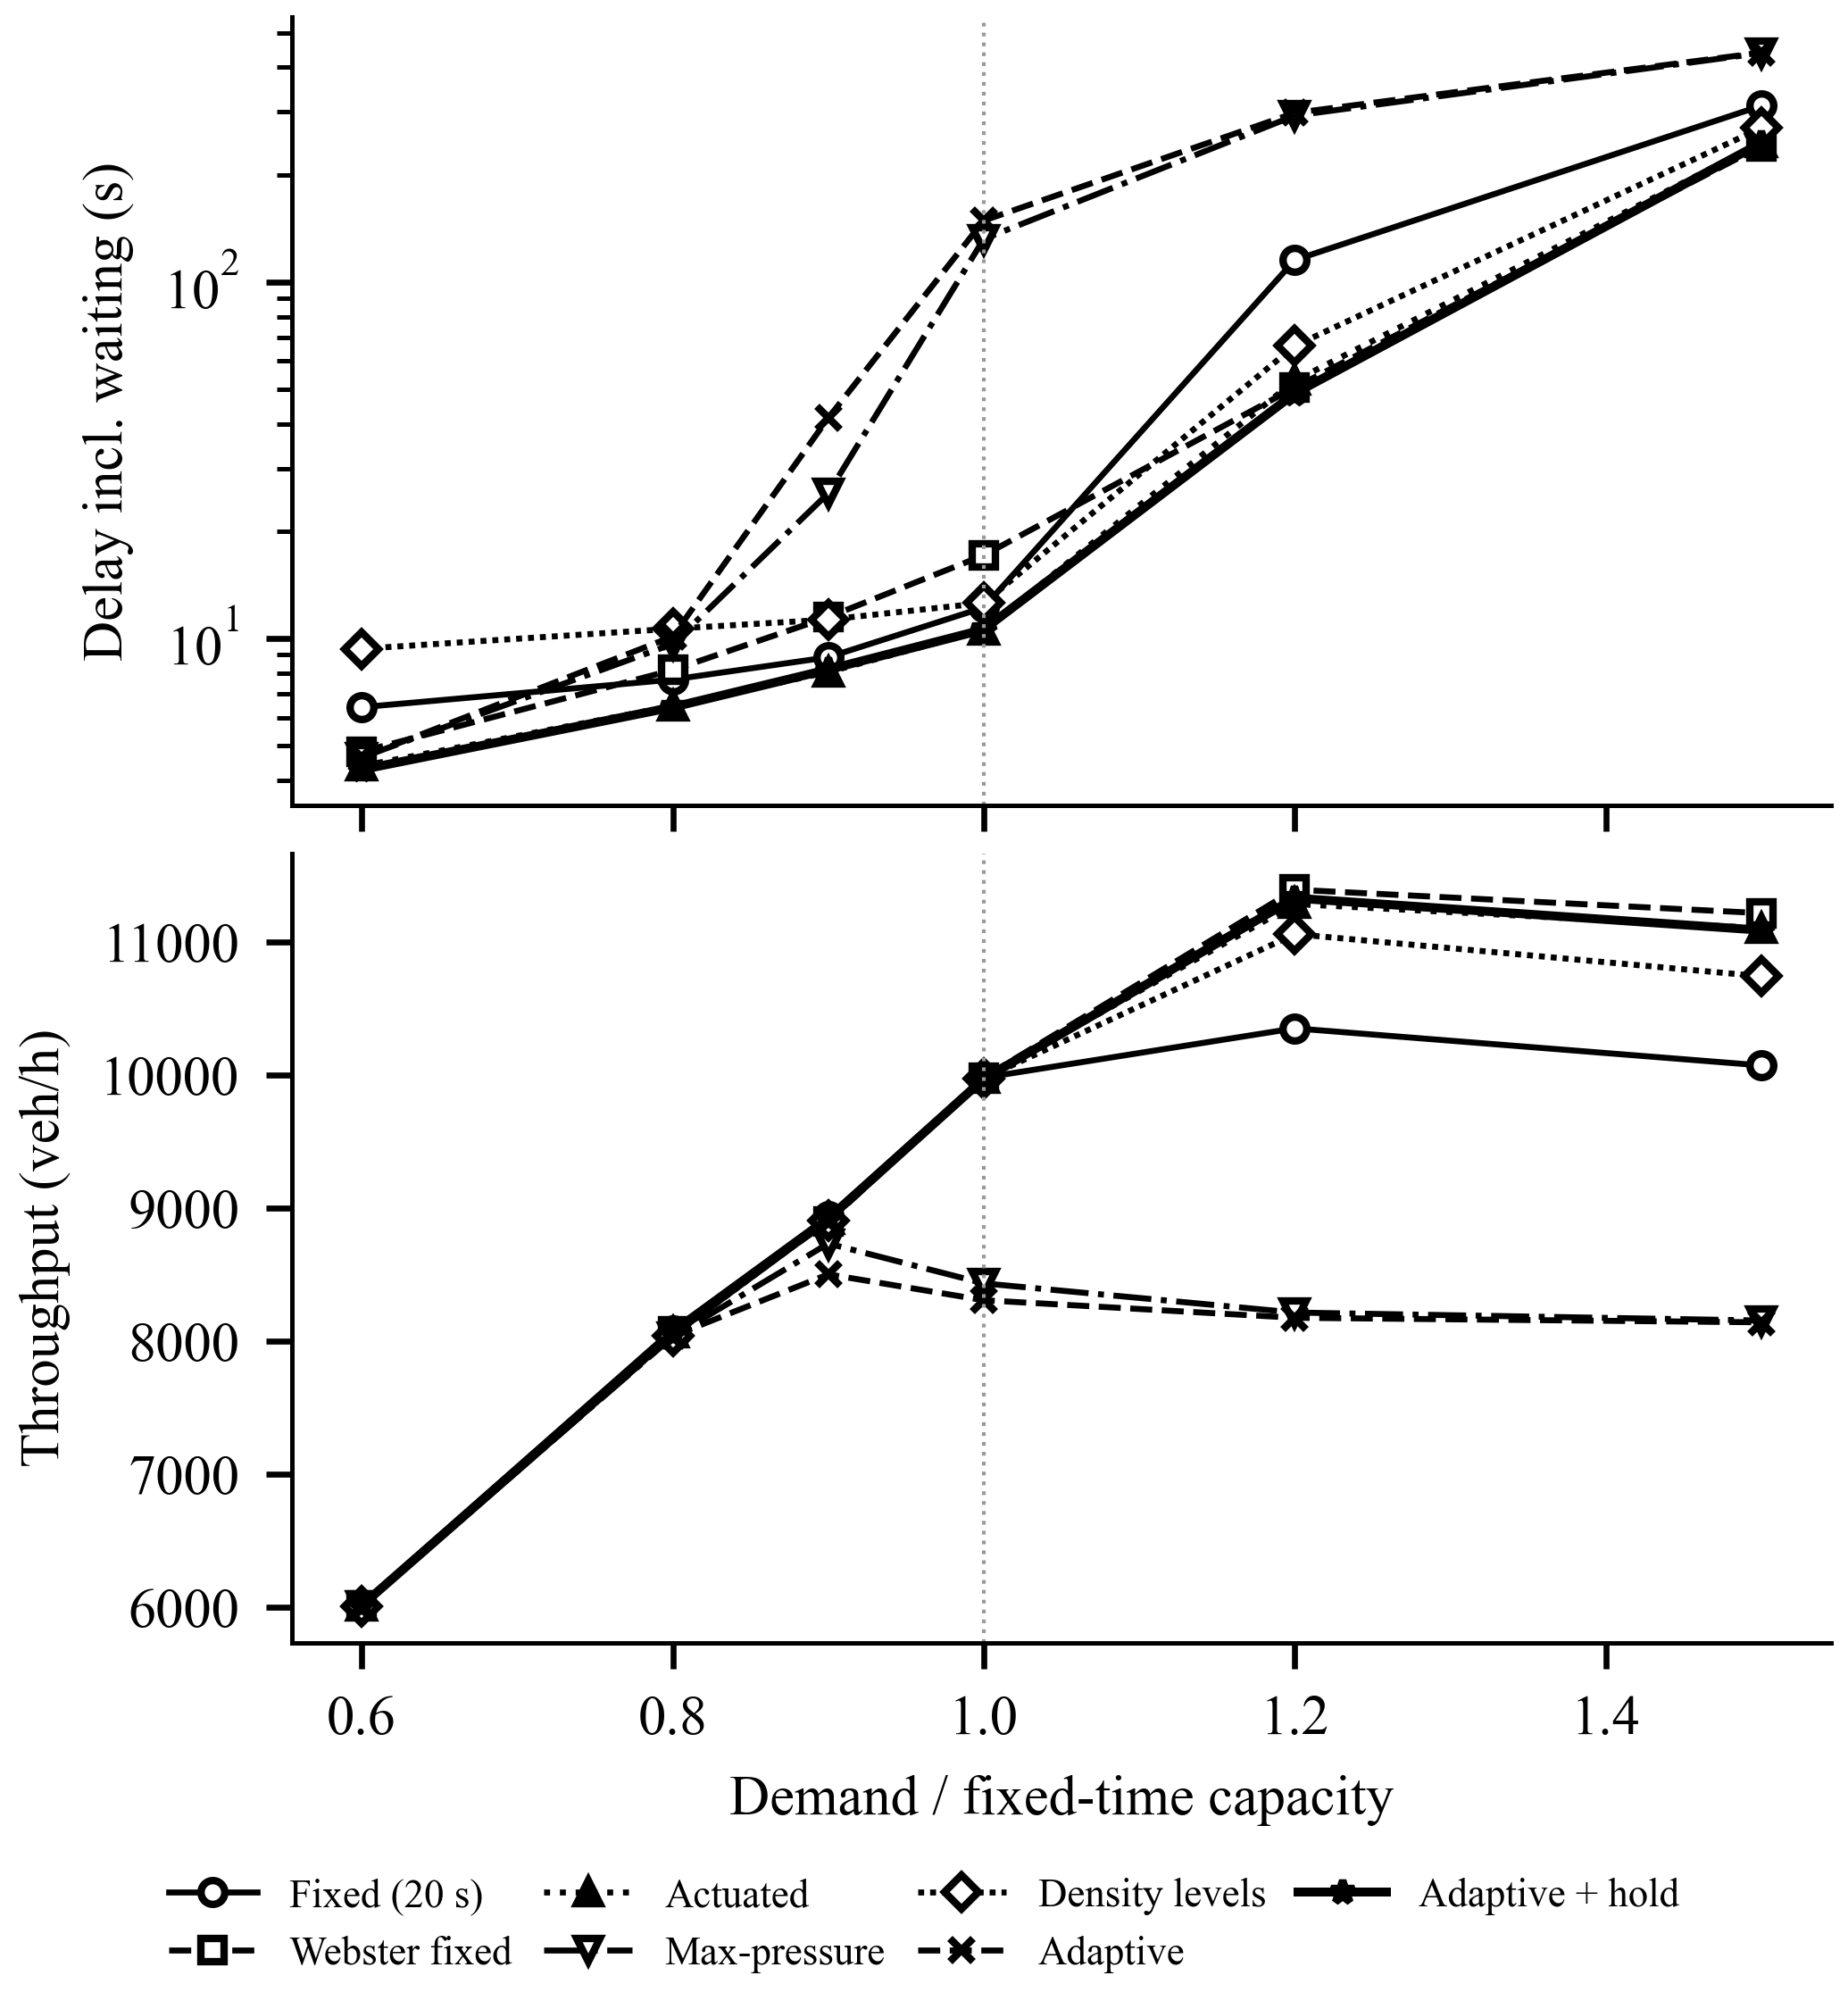
\includegraphics[width=0.7\textwidth]{figures/fig5_above_capacity.png}
\caption{Delay (top, log scale) and throughput (bottom) against demand, preemption off. The dotted line marks the fixed-time capacity.}
\label{fig:above}
\end{figure}


\subsection{Experiment 3: Sixty-Minute Peak Period}
Steady demand shows capacity but not how a controller manages a congestion episode. In a further 60-minute experiment, demand rose from 0.6 to 1.2 times the fixed-time capacity (ramping over 10--15~min), stayed there for 15~min and fell back to 0.6 by 35~min (Figure~\ref{fig:peak}; preemption off, ten paired seeds; the Webster plan timed for the average demand). The queue, including vehicles waiting to enter, peaked at 495 vehicles under fixed timing, 255 with the discharge hold, 254 with actuated control and 1214 with the original adaptive rule. After the peak, the queue returned to its pre-peak level in 13.9 min under fixed timing and 7.3 min with the hold, whereas the original rule did not recover within the hour and max-pressure control 28.7 min (9 of 10 runs did not recover). Approach entries were blocked for 68 approach-minutes under fixed timing, 36 with the hold and 172 with the original rule. During the peak the hold served 11394~veh/h, against 10574 for fixed timing and 8244 for the original rule. Relative to fixed timing, total delay changed by $-$57.3\% with the hold, $-$57.6\% with actuated control and +356.1\% with the original rule. Managing a congestion episode therefore depends above all on not shortening greens while queues are saturated.

\begin{table}[H]
\centering
\caption{Sixty-minute peak period: queue, recovery, spillback, throughput and total delay}
\label{tab:peak}
\small
\resizebox{\ifdim\width>\textwidth\textwidth\else\width\fi}{!}{%
\begin{tabular}{lccccc}
\toprule
\textbf{Controller} & \textbf{Peak queue (veh)} & \textbf{Time to recover} & \textbf{Blocked (approach-min)} & \textbf{Peak throughput (veh/h)} & \textbf{Total delay vs fixed} \\
\midrule
Fixed (20 s) & 495 & 13.9 min & 68 & 10574 & --- \\
Webster fixed & 444 & 13.1 min & 64 & 10723 & $-$10.5\% \\
Actuated & 254 & 7.4 min & 36 & 11406 & $-$57.6\% \\
Max-pressure & 1166 & 28.7 min (9 of 10 runs did not recover) & 167 & 8374 & +325.6\% \\
Adaptive & 1214 & did not recover within the hour & 172 & 8244 & +356.1\% \\
Adaptive + hold & 255 & 7.3 min & 36 & 11394 & $-$57.3\% \\
\bottomrule
\end{tabular}}
\par\smallskip{\footnotesize Demand ramps from 0.6 to 1.2 times capacity, holds for 15 min and falls back; ten paired seeds; preemption off.}
\end{table}

\begin{figure}[H]
\centering
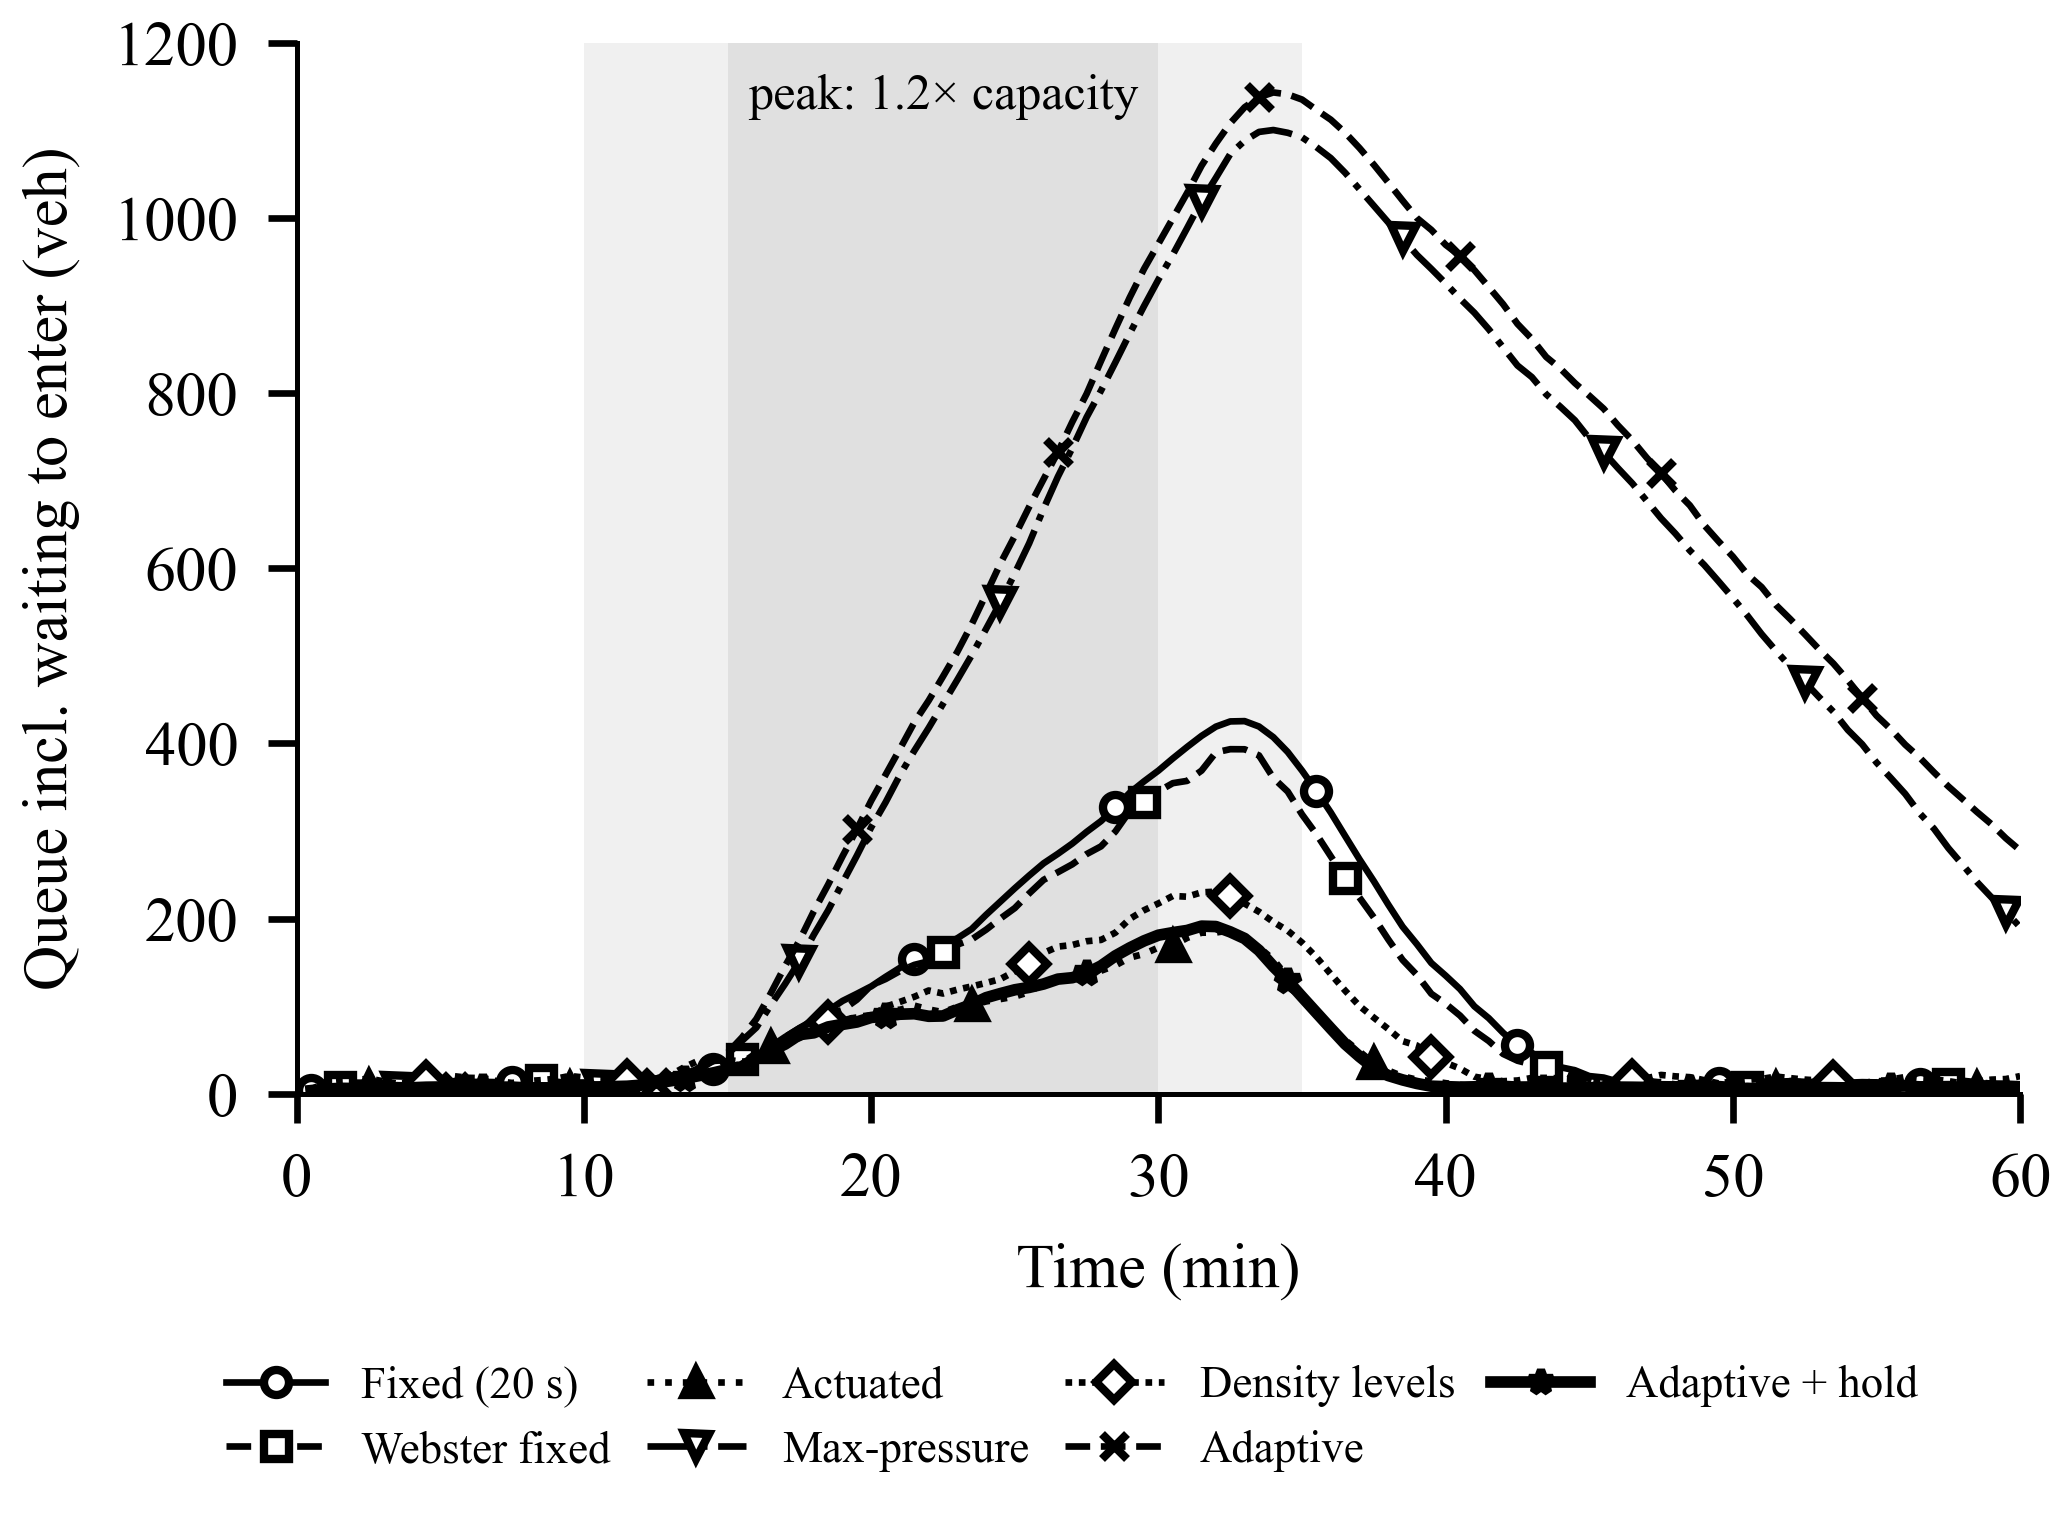
\includegraphics[width=0.85\textwidth]{figures/fig6_peak_queue.png}
\caption{Queue including vehicles waiting to enter during a 60-minute peak period (mean of ten seeds, 2-minute moving average, preemption off). Shading: demand ramping (light) and at 1.2 times the fixed-time capacity (dark).}
\label{fig:peak}
\end{figure}


\subsection{Experiment 4: Emergency Preemption}
Emergency vehicles made up 1\% of arrivals and triggered 12.4--23.4 preemptions per hour under adaptive control (Table~\ref{tab:preemption}). Preemption reduced their mean stopped delay to the start-up component of the metric under every controller (at medium demand from 8.87~s to 0.28~s under fixed timing and from 3.65~s to 0.35~s under adaptive control). The cost to other traffic depends on the controller: at medium demand it was +3.1\% under fixed timing, but +9.3\% under adaptive control and +7.2\% with the hold, because each preemption discards the density-responsive timing and restarts the plan at a fixed phase. Emergency vehicles are far more frequent here than in normal traffic, so the aggregate cost at a real junction would be expected to be smaller.

\begin{table}[H]
\centering
\caption{Effect of emergency preemption}
\label{tab:preemption}
\small
\resizebox{\ifdim\width>\textwidth\textwidth\else\width\fi}{!}{%
\begin{tabular}{llcccc}
\toprule
\textbf{Demand} & \textbf{Controller} & \textbf{EVs off/on} & \textbf{EV delay (s) off$\rightarrow$on} & \textbf{Other delay (s) off$\rightarrow$on} & \textbf{Other change ($p$)} \\
\midrule
Low & Fixed (20 s) & 58/58 & 7.0$\rightarrow$0.28 & 7.06$\rightarrow$7.04 & $-$0.2\% (0.86) \\
Low & Adaptive & 58/58 & 2.42$\rightarrow$0.28 & 4.34$\rightarrow$4.54 & +4.5\% ($<$ 0.001) \\
Low & Adaptive + hold & 58/58 & 2.5$\rightarrow$0.28 & 4.32$\rightarrow$4.49 & +3.8\% (0.003) \\
Medium & Fixed (20 s) & 75/74 & 8.87$\rightarrow$0.28 & 7.05$\rightarrow$7.27 & +3.1\% (0.08) \\
Medium & Adaptive & 72/72 & 3.65$\rightarrow$0.35 & 4.25$\rightarrow$4.64 & +9.3\% ($<$ 0.001) \\
Medium & Adaptive + hold & 74/73 & 3.77$\rightarrow$0.3 & 4.35$\rightarrow$4.66 & +7.2\% (0.01) \\
High & Fixed (20 s) & 103/111 & 6.0$\rightarrow$0.42 & 7.28$\rightarrow$7.43 & +2.1\% (0.17) \\
High & Adaptive & 103/105 & 4.18$\rightarrow$0.51 & 4.22$\rightarrow$4.81 & +13.8\% ($<$ 0.001) \\
High & Adaptive + hold & 103/103 & 3.7$\rightarrow$0.57 & 4.41$\rightarrow$4.93 & +11.8\% ($<$ 0.001) \\
\bottomrule
\end{tabular}}
\par\smallskip{\footnotesize EV: emergency vehicles measured, pooled over ten seeds. Other change: paired change in the mean delay of all other vehicles; paired $t$-test $p$-value in parentheses.}
\end{table}


\subsection{Experiment 5: Ablation}
\label{sec:ablation}
Table~\ref{tab:ablation} changes one part of the controller at a time, on the same paired seeds. Counting vehicles without weights or multipliers raised delay by 22.7\% and 26.6\% at medium and high demand. Removing the parts separately shows where this comes from: without the queued/moving distinction delay rose by 35.1\% and 33.0\%, whereas setting every class weight to 1 changed it by $-$3.9\% and $-$3.2\%. The benefit of the score therefore comes from distinguishing queued from moving vehicles, not from the class weights, which did not help as set. Raising $\theta$ to 1.5 lowered delay slightly ($-$4.9\% and $-$4.1\%) and $\theta = 1.0$ made no difference; the discharge hold, with any zone length, did not change delay below capacity, where its benefit is not needed.

\begin{table}[H]
\centering
\caption{Ablation of the adaptive controller}
\label{tab:ablation}
\small
\resizebox{\ifdim\width>\textwidth\textwidth\else\width\fi}{!}{%
\begin{tabular}{llcccc}
\toprule
\textbf{Variant} & \textbf{Demand} & \textbf{Mean delay (s)} & \textbf{Change} & \textbf{$p$} & \textbf{Green (s)} \\
\midrule
Adaptive (reference) & medium & 4.60 $\pm$ 0.14 & --- & --- & 9.5 \\
Unweighted count (weights and multipliers = 1) & medium & 5.65 $\pm$ 0.16 & +22.7\% & $<$ 0.001 & 14.1 \\
No class weights (all classes = 1) & medium & 4.42 $\pm$ 0.14 & $-$3.9\% & 0.07 & 8.9 \\
No queued/moving distinction (multipliers = 1) & medium & 6.22 $\pm$ 0.21 & +35.1\% & $<$ 0.001 & 15.1 \\
theta = 1.0 & medium & 4.66 $\pm$ 0.13 & +1.3\% & 0.39 & 10.0 \\
theta = 1.5 & medium & 4.38 $\pm$ 0.13 & $-$4.9\% & 0.005 & 8.8 \\
+ discharge hold, 10 m zone & medium & 4.62 $\pm$ 0.16 & +0.4\% & 0.82 & 9.7 \\
+ discharge hold, 20 m zone & medium & 4.66 $\pm$ 0.14 & +1.3\% & 0.44 & 9.8 \\
+ discharge hold, 30 m zone & medium & 4.61 $\pm$ 0.12 & +0.2\% & 0.92 & 10.5 \\
Preemption off & medium & 4.24 $\pm$ 0.09 & $-$7.8\% & $<$ 0.001 & 9.2 \\
Fixed 20 s (for reference) & medium & 7.20 $\pm$ 0.20 & +56.5\% & $<$ 0.001 & 19.6 \\
Adaptive (reference) & high & 4.76 $\pm$ 0.12 & --- & --- & 9.5 \\
Unweighted count (weights and multipliers = 1) & high & 6.03 $\pm$ 0.19 & +26.6\% & $<$ 0.001 & 14.3 \\
No class weights (all classes = 1) & high & 4.61 $\pm$ 0.15 & $-$3.2\% & 0.04 & 9.1 \\
No queued/moving distinction (multipliers = 1) & high & 6.34 $\pm$ 0.15 & +33.0\% & $<$ 0.001 & 15.0 \\
theta = 1.0 & high & 4.75 $\pm$ 0.14 & $-$0.3\% & 0.84 & 9.8 \\
theta = 1.5 & high & 4.57 $\pm$ 0.14 & $-$4.1\% & 0.06 & 8.9 \\
+ discharge hold, 10 m zone & high & 4.89 $\pm$ 0.23 & +2.5\% & 0.17 & 9.7 \\
+ discharge hold, 20 m zone & high & 4.87 $\pm$ 0.15 & +2.2\% & 0.06 & 10.0 \\
+ discharge hold, 30 m zone & high & 4.94 $\pm$ 0.19 & +3.6\% & 0.09 & 10.9 \\
Preemption off & high & 4.22 $\pm$ 0.06 & $-$11.4\% & $<$ 0.001 & 8.9 \\
Fixed 20 s (for reference) & high & 7.36 $\pm$ 0.22 & +54.5\% & $<$ 0.001 & 19.3 \\
\bottomrule
\end{tabular}}
\par\smallskip{\footnotesize Preemption enabled unless stated; ten paired seeds per row; change relative to the reference at the same demand.}
\end{table}


\subsection{Experiment 6: Vision Pipeline Accuracy and Failure Cases}
The vision pipeline was evaluated on seeds 1--4 (9,600 frames, 14,874 vehicle instances in view). On these synthetic frames the generic cascade performed poorly: precision was 4.1\% and recall 8.2\% (Table~\ref{tab:detector}). The failure cases are systematic. 98.6\% of the false positives recur at the same spot in at least 10\% of a camera's frames, i.e.\ the cascade fires on fixed background texture rather than on vehicles. Recall varies by class (car 7.1\%, motorcycle 11.8\%, auto 7.6\%, bus 7.2\%, truck 7.7\%, fire\_truck 3.7\%, ambulance 14.3\%) and by distance from the stop line (0-20 m 5.4\%, 20-40 m 16.9\%, 40-60 m 17.4\%); recall is lowest near the stop line, where queued vehicles stand close together. Without upscaling, or without histogram equalization, the cascade found essentially nothing. A 2$\times$ instead of 3$\times$ upscale raised precision to 63.3\% but cut recall to 3.7\%, so no setting of this generic cascade gives both.

\begin{table}[H]
\centering
\caption{Detector accuracy and ablation (synthetic frames)}
\label{tab:detector}
\small
\resizebox{\ifdim\width>\textwidth\textwidth\else\width\fi}{!}{%
\begin{tabular}{lccc}
\toprule
\textbf{Detector variant} & \textbf{Precision (\%)} & \textbf{Recall (\%)} & \textbf{Detections per frame} \\
\midrule
Default (3x upscale, equalized) & 4.1 & 8.2 & 3.30 \\
2x upscale & 63.3 & 3.7 & 0.09 \\
No upscaling & --- & 0.0 & 0.00 \\
No histogram equalization & --- & 0.0 & 0.00 \\
\bottomrule
\end{tabular}}
\par\smallskip{\footnotesize Pooled over seeds 1--4; a detection is correct when its centre lies inside a ground-truth box enlarged by 4 px. ---: too few detections for a meaningful precision.}
\end{table}


Tracking was evaluated on the default detector's output (Table~\ref{tab:tracking}). Only 0.6\% of the vehicle instances in view carried a confirmed track, and 1.5\% of the vehicles were confirmed at least once. For confirmed tracks on real vehicles, the mean absolute error of the tracked speed was 0.53~m/s over 82 estimates. This is not a good result: the vehicles concerned were moving at only 0.56~m/s on average, because tracks are confirmed almost only on nearly stationary, queued vehicles, so the error is as large as the speed itself and the pipeline provides no usable kinematics for moving traffic. Dropping the low-confidence second matching stage or the motion model changed coverage little, because the limiting factor is the detector's recall, not the association. These results are why the evaluated controllers read vehicle states from the simulator: a class-aware detector trained on the target imagery is needed before detections can drive control, and accuracy on real footage is unknown.

\begin{table}[H]
\centering
\caption{Tracking quality and tracked-speed error}
\label{tab:tracking}
\small
\resizebox{\ifdim\width>\textwidth\textwidth\else\width\fi}{!}{%
\begin{tabular}{lcccc}
\toprule
\textbf{Tracker variant} & \textbf{Coverage (\%)} & \textbf{Vehicles confirmed (\%)} & \textbf{ID switches / 100 veh.} & \textbf{Speed MAE (m/s)} \\
\midrule
ByteTrack-style (two-stage, Kalman) & 0.6 & 1.5 & 0.2 & 0.53 \\
Single stage (low-confidence dropped) & 0.5 & 1.0 & 0.2 & 0.16 \\
No motion model (last box) & 0.6 & 1.5 & 0.2 & n/a \\
Confirm after 1 match & 2.3 & 35.9 & 6.6 & 0.53 \\
\bottomrule
\end{tabular}}
\par\smallskip{\footnotesize Coverage: share of vehicle instances in view with a confirmed track. Speed MAE: confirmed tracks on real vehicles with at least three matches; n/a where the variant has no motion estimate.}
\end{table}


\subsection{Experiment 7: Validation of the Simulated Kinematics}
\label{sec:kin}
To check the simulator's kinematics against external values, queue discharge was measured as at a real junction: the time between successive queued vehicles crossing the stop line after the green starts, in saturated fixed-time runs (five seeds). The Highway Capacity Manual's base values are 1900 passenger cars per hour per lane (a 1.89~s headway) and a start-up lost time of about 2~s~\cite{ref24}. The model used for the main results discharges cars every 0.51~s (7,102~veh/h/lane; Table~\ref{tab:kinematics}): without a reaction time a follower may trail by only the 2~m standstill gap at any speed. Adding a driver reaction time $\tau$ to the safe speed, as in Krau{\ss}'s model~\cite{ref25}, and setting $\tau = 1.6$~s gives 1.92~s (1,877~veh/h/lane) for cars, within 1.2\% of the reference. The calibrated model still has no extra delay when a queue starts to move, so its start-up lost time ($-$0.8~s) is lower than in the field.

\begin{table}[H]
\centering
\caption{Queue discharge against field reference values}
\label{tab:kinematics}
\small
\resizebox{\ifdim\width>\textwidth\textwidth\else\width\fi}{!}{%
\begin{tabular}{lcccc}
\toprule
\textbf{Model} & \textbf{Headway, cars (s)} & \textbf{Sat. flow, cars (veh/h/lane)} & \textbf{Sat. flow, all (veh/h/lane)} & \textbf{Start-up lost time (s)} \\
\midrule
Simulator, $\tau$ = 0 (used for main results) & 0.51 & 7,102 & 3,164 & 2.1 \\
Simulator, $\tau$ = 1.6 s (calibrated) & 1.92 & 1,877 & 1,798 & -0.8 \\
HCM base values [24] & 1.89 & 1,900 & --- & $\approx$ 2.0 \\
\bottomrule
\end{tabular}}
\par\smallskip{\footnotesize Saturated fixed-time runs, five seeds; saturation headway averaged from the fifth queued vehicle on.}
\end{table}


All comparisons were then repeated with the calibrated model ($\tau = 1.6$~s; the Webster plan recomputed with the calibrated saturation flow of 3600~veh/h per approach). Table~\ref{tab:calibrated} summarizes them. Below capacity, the reductions relative to the fixed plan were 33.7--35.4\% for the adaptive controller and 31.9--39.2\%, 35.0--39.5\% and 34.7--38.9\% for the Webster plan, actuated and max-pressure control. The calibrated capacity of the fixed plan was 6,148~veh/h; relative to it, the original adaptive rule reached $-$14.6\% and the Webster plan +6.3\%. The discharge hold, with the 10~m zone chosen for the default model, reached only $-$3.7\% (mean saturated green 17.4~s): with a reaction time, vehicles leaving a queue spread out to gaps of about 20~m at speed, so a 10~m zone empties between them and the green gaps out while the queue is still discharging. The zone is therefore a kinematics-dependent parameter, as the passage time of a real actuated controller is set for local conditions. Re-tuned for the calibrated model on the tuning seed (20.0~m), the discharge hold reached +6.1\% capacity relative to fixed timing and actuated control +6.1\%, against +6.3\% for the Webster plan.

\begin{table}[H]
\centering
\caption{Main comparisons repeated with calibrated kinematics}
\label{tab:calibrated}
\small
\resizebox{\ifdim\width>\textwidth\textwidth\else\width\fi}{!}{%
\begin{tabular}{lcccc}
\toprule
\textbf{Controller} & \textbf{Delay vs fixed, low} & \textbf{medium} & \textbf{high} & \textbf{Capacity vs fixed} \\
\midrule
Webster fixed & $-$38.0\% & $-$39.2\% & $-$31.9\% & +6.3\% \\
Actuated & $-$39.4\% & $-$39.5\% & $-$35.0\% & $-$3.9\% \\
Max-pressure & $-$38.9\% & $-$38.7\% & $-$34.7\% & $-$14.5\% \\
Density levels & +7.4\% & +29.1\% & +31.4\% & +4.1\% \\
Adaptive & $-$35.2\% & $-$35.4\% & $-$33.7\% & $-$14.6\% \\
Adaptive + hold & $-$35.5\% & $-$35.0\% & $-$33.7\% & $-$3.7\% \\
Actuated, zone 20.0 m & $-$39.0\% & $-$38.5\% & $-$32.4\% & +6.1\% \\
Adaptive + hold, zone 20.0 m & $-$34.1\% & $-$34.4\% & $-$32.0\% & +6.1\% \\
\bottomrule
\end{tabular}}
\par\smallskip{\footnotesize $\tau$ = 1.6 s; ten paired seeds per demand level (preemption on) and five capacity seeds (preemption off). Gap-out controllers use the 10 m zone unless a re-tuned zone is stated.}
\end{table}


\subsection{Experiment 8: Imperfect Sensing}
All results so far assume that the controller knows every vehicle's position, speed and class. To measure how much this matters, the vehicle-reading controllers were run behind a sensor model that reports only what a camera would: vehicles within 60~m of the stop line, refreshed at 2~Hz, without classes (as a single cascade), with each vehicle detected independently with a given recall, and optionally with phantom detections at fixed spots, like the cascade's static false positives. The last profile uses the measured pipeline of Experiment 6. Emergency preemption still reads the true emergency flags; ten paired seeds per cell. Tables~\ref{tab:sensing-med} and~\ref{tab:sensing-cap} give the results at medium demand and at 0.9 times capacity. Below capacity the controllers tolerated missed detections well, because missing vehicles only shortens greens, which costs little when queues are short. Near capacity, sensing mattered: the discharge-hold controller's delay rose from 7.8 s with exact states to 8.5 s with a perfect camera view and 14.4 s at 50\% recall, against 8.8 s for the fixed plan. Phantom detections were the most damaging error for the gap-out rule: a phantom inside the 10 m zone never moves, so the green never gaps out and runs to the maximum (medium-demand delay 11.9 s, +64.8\% relative to fixed timing). With the measured pipeline, every vehicle-reading controller was worse than the fixed plan near capacity (discharge hold 162.9 s against 8.8 s). At medium demand max-pressure and adaptive still beat the fixed plan, because phantoms appear on both directions and largely cancel in their comparisons, whereas actuated and adaptive + hold were held at long greens by phantoms in the stop-line zone (11.9 s against 7.2 s). Closing the loop with the present detector would therefore harm traffic; a detector must at least suppress static false positives near the stop line, and its recall matters most near capacity.

\begin{table}[H]
\centering
\caption{Delay under imperfect sensing (s), medium demand}
\label{tab:sensing-med}
\small
\resizebox{\ifdim\width>\textwidth\textwidth\else\width\fi}{!}{%
\begin{tabular}{lcccc}
\toprule
\textbf{Sensing} & \textbf{Actuated} & \textbf{Max-pressure} & \textbf{Adaptive} & \textbf{Adaptive + hold} \\
\midrule
Exact states & 4.4 & 4.3 & 4.6 & 4.6 \\
Camera (60 m, 2 Hz, no classes) & 4.4 (+1.4\%) & 4.3 (+0.4\%) & 4.3 ($-$5.9\%) & 4.4 ($-$5.4\%) \\
recall 90\% & 4.4 (+0.4\%) & 4.4 (+1.0\%) & 4.3 ($-$5.6\%) & 4.3 ($-$6.3\%) \\
recall 70\% & 4.3 ($-$0.1\%) & 4.3 (+0.2\%) & 4.3 ($-$5.4\%) & 4.4 ($-$5.1\%) \\
recall 50\% & 4.4 (+0.4\%) & 4.3 ($-$0.7\%) & 4.3 ($-$5.7\%) & 4.3 ($-$6.2\%) \\
recall 30\% & 4.4 (+0.3\%) & 4.4 (+0.5\%) & 4.4 ($-$5.3\%) & 4.4 ($-$5.6\%) \\
2 phantoms per approach & 11.9 (+172.2\%) & 4.3 (+0.4\%) & 4.3 ($-$5.7\%) & 11.9 (+156.8\%) \\
Measured Haar (recall 8\%, 3 phantoms) & 11.9 (+173.1\%) & 4.7 (+8.1\%) & 4.3 ($-$5.7\%) & 11.9 (+157.6\%) \\
\bottomrule
\end{tabular}}
\par\smallskip{\footnotesize Change relative to the same controller with exact states in brackets. Fixed plan (needs no sensing): 7.2 $\pm$ 0.2 s.}
\end{table}

\begin{table}[H]
\centering
\caption{Delay under imperfect sensing (s), 0.9 times capacity}
\label{tab:sensing-cap}
\small
\resizebox{\ifdim\width>\textwidth\textwidth\else\width\fi}{!}{%
\begin{tabular}{lcccc}
\toprule
\textbf{Sensing} & \textbf{Actuated} & \textbf{Max-pressure} & \textbf{Adaptive} & \textbf{Adaptive + hold} \\
\midrule
Exact states & 8.1 & 27.2 & 35.6 & 7.8 \\
Camera (60 m, 2 Hz, no classes) & 8.5 (+4.6\%) & 30.1 (+10.6\%) & 45.0 (+26.5\%) & 8.5 (+8.4\%) \\
recall 90\% & 8.4 (+3.5\%) & 32.3 (+18.6\%) & 45.4 (+27.5\%) & 8.3 (+5.6\%) \\
recall 70\% & 9.0 (+10.9\%) & 36.4 (+33.8\%) & 45.4 (+27.5\%) & 9.4 (+19.3\%) \\
recall 50\% & 11.3 (+39.8\%) & 33.0 (+21.2\%) & 45.4 (+27.5\%) & 14.4 (+83.9\%) \\
recall 30\% & 20.6 (+154.0\%) & 35.7 (+30.9\%) & 48.6 (+36.5\%) & 23.2 (+195.8\%) \\
2 phantoms per approach & 15.1 (+86.2\%) & 30.1 (+10.6\%) & 45.0 (+26.5\%) & 15.1 (+92.0\%) \\
Measured Haar (recall 8\%, 3 phantoms) & 163.3 (+1915.8\%) & 33.2 (+21.9\%) & 45.2 (+27.0\%) & 162.9 (+1973.7\%) \\
\bottomrule
\end{tabular}}
\par\smallskip{\footnotesize Delay includes time waiting to enter the road; preemption off. Fixed plan: 8.8 $\pm$ 0.2 s.}
\end{table}


\subsection{Experiment 9: Calibration of the Density Weights}
\label{sec:calib}
The class weights and multipliers of Eq.~\eqref{eq:density} were set by hand. To calibrate them from data, a random search over the score parameters of the discharge-hold controller (four class weights and the emergency-vehicle weight, log-uniform 0.25--4 and 1--10; the queued/moving ratio, 1--12; and $\theta$, 1.0--1.6; the car weight stays 1 because rule~\eqref{eq:green} compares ratios) evaluated 14 candidates on tuning seeds 1001--1002 at medium demand, high demand and 0.9 times capacity, minimizing delay relative to the hand-set weights. The best candidate (motorcycle 1.89, auto-rickshaw 3.02, bus 1.67, truck 0.93, emergency 1.91, queued/moving ratio 2.94, $\theta$ = 1.37), the hand-set weights and a plain vehicle count were then compared on the held-out seeds 1--10 (Table~\ref{tab:calibration}). On the held-out seeds the calibrated score changed delay by $-$2.0\% (medium, $p$ = 0.374), $-$4.9\% (high, $p$ = 0.036), +2.2\% (0.9x capacity, $p$ = 0.014) relative to the hand-set weights, whereas a plain vehicle count was worse by +23.2\%, +22.7\%, +13.4\% respectively. The plain count remained clearly worse, confirming the ablation. The calibrated parameters are fitted to this simulator's traffic and must be re-fitted against field data before deployment; the search is a simple, reproducible way to do so, not a learned controller.

\begin{table}[H]
\centering
\caption{Calibrated score parameters and held-out delay}
\label{tab:calibration}
\small
\resizebox{\ifdim\width>\textwidth\textwidth\else\width\fi}{!}{%
\begin{tabular}{lccc}
\toprule
\textbf{Parameter / condition} & \textbf{Hand-set} & \textbf{Calibrated} & \textbf{Plain count} \\
\midrule
Motorcycle weight & 0.50 & 1.89 & 1.00 \\
Auto-rickshaw weight & 0.80 & 3.02 & 1.00 \\
Bus weight & 3.00 & 1.67 & 1.00 \\
Truck weight & 2.50 & 0.93 & 1.00 \\
Emergency-vehicle weight & 6.00 & 1.91 & 1.00 \\
Queued/moving ratio & 3.00 & 2.94 & 1.00 \\
Switching ratio $\theta$ & 1.10 & 1.37 & 1.10 \\
Delay, medium (s) & 4.62 & 4.53 ($-$2.0\%, $p$ 0.374) & 5.69 (+23.2\%) \\
Delay, high (s) & 4.89 & 4.64 ($-$4.9\%, $p$ 0.036) & 5.99 (+22.7\%) \\
Delay, 0.9x capacity (s) & 7.85 & 8.03 (+2.2\%, $p$ 0.014) & 8.90 (+13.4\%) \\
\bottomrule
\end{tabular}}
\par\smallskip{\footnotesize Delays on held-out seeds 1--10 (ten paired seeds); changes and $p$ relative to the hand-set weights.}
\end{table}


\section{Discussion}
Two results qualify the usual claim that density-based control beats fixed timing. Below capacity, the gain over an untuned 20~s plan is real but not specific to density scoring: a Webster plan tuned to the demand, actuated control and max-pressure control achieve the same. Near capacity, density-only switching is worse than fixed timing, because it ends greens while the served queue is still discharging. With the discharge hold, the proposed controller matches the best strategies below capacity and comes close to the highest capacity measured (the Webster plan's, +11.6\%), while keeping the properties that motivated it: its decisions follow a rule that can be stated in one line, its red time is bounded in closed form, and its safety is audited at every step. Its results are, however, almost identical to plain actuated control, which uses no density score at all: in this setting the gap-out test, not the score, does most of the work. The score's remaining role is to decide when a cleared green should hand over, where the ablation shows that the queued/moving distinction matters. Emergency priority and adaptive control interact: resuming after preemption with the higher-scoring direction, rather than always the held one, is a direct improvement to test.

The research questions of Section~\ref{sec:contrib} are answered as follows: variable greens keep safe change intervals (no violation in 3,524 runs); preemption serves emergency vehicles without delay but costs other traffic more under adaptive control than under fixed timing; near and above capacity the original rule fails and the hold corrects it; and a large part of the gain below capacity comes from replacing an untuned plan, not from the density score.

\section{Comparison with Existing Work}
Table~\ref{tab:comparison} compares the proposed controller with re-implementations of the strategies used by existing work, which share its phase sequence, change intervals and green limits. The original papers could not be compared directly, since they use different simulators, demands and metrics.

\begin{table}[H]
\centering
\caption{Comparison with the strategies of existing work (re-implemented in the same simulator)}
\label{tab:comparison}
\small
\resizebox{\ifdim\width>\textwidth\textwidth\else\width\fi}{!}{%
\begin{tabular}{lccc}
\toprule
\textbf{Method} & \textbf{Delay, high demand (s)} & \textbf{Capacity vs fixed} & \textbf{Source year} \\
\midrule
Fixed 20 s plan & 7.36 $\pm$ 0.22 & --- & Baseline \\
Webster-optimized plan [2] & 4.60 $\pm$ 0.29 & +11.6\% & 1958 \\
Vehicle-actuated [23] & 4.63 $\pm$ 0.17 & +9.6\% & 2008 \\
Max-pressure [11] & 4.62 $\pm$ 0.18 & $-$18.8\% & 2013 \\
Three-level density control [1] & 9.49 $\pm$ 0.15 & +6.3\% & 2025 \\
Adaptive (density score) & 4.76 $\pm$ 0.12 & $-$18.9\% & \textbf{2026} \\
\textbf{Adaptive + discharge hold (ours)} & 4.89 $\pm$ 0.23 & +9.8\% & \textbf{2026} \\
\bottomrule
\end{tabular}}
\par\smallskip{\footnotesize All methods share the phase sequence, change intervals and 8--45 s green limits; delay from Table~\ref{tab:below}, capacity from Table~\ref{tab:capacity}.}
\end{table}


\section{Limitations}
\begin{itemize}
  \item \textbf{Simulation only.} The model has no turning movements, lane changes, pedestrians or driver variability and has not been calibrated against field data, so absolute delays are not field predictions.
  \item \textbf{Kinematics.} The model behind the main results has no driver reaction time, so its queues discharge much faster than real ones. A reaction time of 1.6~s matches the field saturation headway, but the calibrated model still lacks start-up delay, so its start-up lost time is too low; with real start-up lost time, short greens would cost more, so the original rule's capacity loss is if anything understated. The gap-out zone of the discharge hold must also suit the local vehicle spacing: 10~m for the default model, 20.0~m for the calibrated one.
  \item \textbf{Arrival model.} Arrivals follow deterministic headways at a rate redrawn every 15~s, not a Poisson process, and emergency vehicles are far more frequent than in real traffic.
  \item \textbf{Comparison controllers.} The baselines are re-implementations of the published strategies with ideal sensing, not the original systems; the Webster plan is given the true mean demand of each run.
  \item \textbf{Sensing.} The main results use exact vehicle states, and emergency vehicles are detected perfectly. The controllers need a detector far better than the present Haar pipeline, in particular one without static false positives near the stop line. The vision pipeline was tested only on synthetic frames; real footage with lighting changes, occlusion and weather is harder.
  \item \textbf{Parameters and hardware.} The calibrated score parameters are fitted to this simulator, not to field data; the congestion thresholds used for display were set by hand. A planned Raspberry Pi 4 deployment, with one camera per approach and relay-driven signal heads, is estimated at roughly INR 6,000--8,000 in components, and its detection time at 5--10 times slower than the laptop; these are estimates and must be verified on actual hardware.
\end{itemize}
